\chapter{A brief introduction to electric charges, currents, fields and potentials} 
\label{sec:Basics}
Action potentials are generated by electric currents over neural membranes. In turn, these currents
evoke the extracellular electric potentials that are the main topic of this book. 

Before we talk more about the electric signaling in the brain, we will in this chapter give a general introduction to the physics of electricity. The aim of this rather incomplete introduction is to establish an elementary understanding of the main concepts that we will use in the remainder of this book. Readers without prior schooling in physics will probably not be able to follow all parts of it, but it will hopefully still give them a basic understanding of the concepts of \textit{electric charge}, \textit{electic currents}, \textit{electric fields}, and \textit{electric potentials}, and some insight into how they are related to one another. Readers that do have a physics background might see it as a useful repetition. 

Most of the physics that we will go through is summarized in, and follows from, Maxwell's equations, and we might have kick-started this chapter by listing up those. However, since Maxwell's equations may appear a bit challenging for "the untrained eye", we will be taking a "softer" path, which we deem sufficient for establishing the main concepts that we will be working with. For good taste and later reference, we nevertheless go through Maxwell's equations in the final part of the chapter (Section \ref{sec:Basics:Maxwell}).


\section{\orange{GH: Electric charge}}
\label{sec:Basics:Charge} \index{Charge}
Let us begin with the fundamental quantity for electricity, the electric charge. Nature's fundamental charges are those carried by the protons and electrons that build up the atoms that build up the material world. The proton carries the charge $e$, while the electron has carries the charge $-e$, where $e = 1.602\times10^{-19}$ Coulomb (C) is called the \textit{unit charge} \index{Unit charge}. 

Since atoms contain an equal number of electrons and protons, most matter is electrically neutral. Some mediums are nevertheless conductive, which means that they contain so-called "free charge carriers" that may move through the medium. In an electric copper cable, such as that powering a lamp in a in a normal house, the free charge carriers are electrons that are not bound to specific locations (i.e., to specific copper atoms), but can move freely through the copper material. In an electrolyte solution, for example salt-water, the free charge carriers are instead ions, i.e., atoms or molecules that have gained or donated one or several electrons, and therefore have become electrically charged. The saline solutions that fill the intracellular and extracellular space of the brain are such electrolytic solutions. Important charge carriers in the brain are sodium and potassium ions (Na$^+$ and K$^+$ with charge $1e$), chloride ions (Cl$^-$ with charge $-1e$), and calcium ions (Ca$^{2+}$ with charge $2e$).

At a fundamental, microscopic level, electricity is largely due to the interactions between individual charges. A pair of charges, $q$ and $q'$, 
\ehnote{Inkonsistent notasjon med det som kommer etter. 
Ville valgt $q_1$, $q_2$ ogsaa her.}
will act on each others with a force $F$, with units Newton (N) given by Coulomb's law:
\begin{equation}
F = k_e qq' \frac{1}{r^2}, 
\label{Basics:eq:CoulombF}
\end{equation}
where $k_e = 8.99\times10^9$ N$\cdot$ m$^2\cdot$C$^{-2}$ is Coulomb's constant, and $r$ is the distance between the two charges. The direction of the force is along the line between the two charges, and the force is inversely proportional to the square of the distance between them. The force will be repelling if the charges have the same valency (sign) and attractive if they have the opposite valency. 

We can express the direction of the force mathematically by use of a vector notation. Letting a boldface notation indicate that an entity is a vector, we may denote the positions of the charges $q$ and $q'$ by ${\bf r}$ and ${\bf r'}$, respectively. The position vector ${\bf r}$ can be visualized as an arrow from some reference point $r=0$ to the position of the charge $q$. Likewise, the vector ${\bf r}-{\bf r'}$ can be visualized from the position of $q'$ to the position of $q$, defining both the distance and direction of the (imagined) line connecting them. In vector notation, the force between the charge pair can be written:
\begin{equation}
{\bf F} = k_e q q' \frac{{\bf r}-{\bf r'}}{|{\bf r}-{\bf r'}|^3} = k_e  qq'  \frac{1}{|{\bf r}-{\bf r'}|^2} \frac{{\bf r}-{\bf r'}}{|{\bf r}-{\bf r'}|}.
\label{Basics:eq:CoulombFvec}
\end{equation}
Here, $|{\bf r}-{\bf r'}|$ denotes the length of the vector ${\bf r}-{\bf r'}$, i.e., the distance between the two charges, cf., $r$ in eq. \ref{Basics:eq:CoulombF}. In the rightmost expression, we have tried to illustrate the similarity to \ref{Basics:eq:CoulombF} expressing the splitting the magnitude and the direction of the force into two factors. The scalar factor $(k_e qq')/|{\bf r}-{\bf r'}|^2$ determines the force magnitude, and is the same as in eq. \ref{Basics:eq:CoulombF}. The remaining factor, $({\bf r}-{\bf r'})/|{\bf r}-{\bf r'}|$ is the division of a vector by its own length, and defines a \textit{unit vector}, a vector with length 1 defining the direction between the positions ${\bf r}$ and ${\bf r'}$, and thus of the force. 

If there are several ($N$) point charges present, the contribution from each of them sum up linearly. If we have a charge $q$ in a position ${\bf r}$, the force acting on it by the $N-1$ other charges $q_1, q_2, q_3 ... q_{N-1}$ in positions ${\bf r_1}, {\bf r_2}, {\bf r_3} ... {\bf r_{N-1}}$ 
\ehnote{subfix skal ikke vaere boldfont.} 
will then be:
\begin{equation}
{\bf F}({\bf r}) = \sum_{n=1}^{N-1} k_e q q_n \frac{{\bf r}-{\bf r_n}}{|{\bf r}-{\bf r_n}|^3}.
\label{Basics:eq:CoulombFN}
\end{equation}

If our system of study consisted of a small number $N$ of charges, we could use $N$ instances of eq. \ref{Basics:eq:CoulombFN} to compute the force acting on all the $N$ individual charges. Together with Newton's law ${\bf F} = m {\bf a}$, which tells us how the charges will be accelerated in the force direction, eq.\ref{Basics:eq:CoulombFN} would then allow us to compute the movements of all our charges over time. 

There is a fairly long way to go from eq. \ref{Basics:eq:CoulombF} to the understanding of electric phenomena in a macroscopic system such as for example the brain. When describing a macroscopic system, we are usually not interested in the microscopic interactions between a small number of charges, but rather the joint interactions of a very, very large number of charges. It is then not feasible to keep track of the motion of each individual charge. At the larger scale, we therefore do not want to work with forces acting on individual particles, but rather with the concept of electric fields, which we will define below. It is still nice to have taken a look at  Eq. \ref{Basics:eq:CoulombFN}, since it establishes the fundamental origin of electrical forces and fields. 


\section{\orange{GH: Electric fields}}
\label{sec:Basics:Fields} \index{Electric field}
The electric field at a given location (measured in volts per meter (V/m)) can be defined as the force that will act on a reference charge $q$ present there, i.e., 
\begin{equation}
{\bf E}({\bf r}) = {\bf F}({\bf r})/q.
\label{Basics:eq:E}
\end{equation}
If we assume that this force is exclusively due to the Coulomb interaction between electric charges, the electric field can be obtained by inserting eq. \ref{Basics:eq:CoulombFN} into eq. \ref{Basics:eq:E}:
\begin{equation}
{\bf E}({\bf r}) = \sum_{n=1}^{N-1} k_e q_n \frac{{\bf r}-{\bf r_n}}{|{\bf r}-{\bf r_n}|^3}.
\label{Basics:eq:CoulombEN}
\end{equation}

Like eq. \ref{Basics:eq:CoulombFN}, eq. \ref{Basics:eq:CoulombEN} applies to a microscopic level, meaning that the field predicted by it will be big at locations that are close to an individual charge (i.e., at all locations where $|{\bf r}-{\bf r_n}|$ is small), and smaller at points where the distance to the nearest charge is longer. Since the average distance between ions in the saline solution of the brain is on the order of a nanometer, this means that the field will vary with a sub-nanometer resolution. A direct use of eq. \ref{Basics:eq:CoulombEN} will therefore, again, force us to keep track of each individual charge, which would not be feasible in a macroscopic system.

Fortunately, we do not have to care too much about these microscopic field variations when we are trying to understand the brain. A technical argument for why this is not the case, is that the electrodes used to record brain signals have a tip diameter which is typically a micrometer or more. This is much, much larger than the average intra-charge distance in the saline solution of the brain. The electrodes therefore do not "see" the microscopic fluctuations, but rather sense the average field taken over the electrode surface. When we speak of an electric field or electric potential in the brain, we therefore always mean field or potential on a so-called \textit{coarse-grained} scale, averaged over an electrode surface of at least $1 \mu$m$^2$. A non-technical argument is that it is this coarse-grained signal, and not the microscopic reality that is bubbling underneath it, that is of importance if we want to understand the key brain processes. 

From here on, we shall not think of ${\bf E}$ as something that we compute based on
knowledge of the microscopic charge distribution (cf. eg. \ref{Basics:eq:CoulombEN}), but rather as a higher level entity, exerting an average force on all charges in a certain direction.


\section{\orange{GH: Electric potentials}}
\label{sec:Basics:Potential} \index{Electric potential}
Tightly related to the electric field ${\bf E}$ is the electric potential $\phi$ (with units volt (V)), which is what we normally measure experimentally when we stick an electrode into the brain. While ${\bf E}$ is a fundamental physical entity, $\phi$ may be regarded as an auxiliary variable. It is a way to represent the electric field that often makes computations simpler and measurements easier. 

The electric field can be expressed as the spatial derivative, or gradient, of the potential:
\begin{equation}
{\bf E}(x,y,z) = - \nabla \phi(x,y,z) = - \left(\frac{d\phi}{dx} {\bf e_x}  + \frac{d\phi}{dy} {\bf e_y} + \frac{d\phi}{dz} {\bf e_z} \right) \phi.
\label{Basics:eq:EV}
\end{equation}
The operator $\nabla$ computes a property's spatial rate of change in the various spatial directions, and ${\bf e_x}$, ${\bf e_y}$ and  ${\bf e_z}$ are the unit vectors in the three spatial directions $x$, $y$ and $z$, respectively. Unlike ${\bf E}$, which is a vector-field, $\phi$ is a scalar function, and as such, it tends to be easier to deal with. We note that eq. \ref{Basics:eq:EV} rests on something called the \textit{quasi-static approximation} of Maxwell's equations, which we explain further in Section \label{sec:Basics:Maxwell}. 

\subsection{\orange{GH: Electric ground}}
To get an intuitive understanding of the relationship between ${\bf E}$ and $\phi$, it helps to consider an idealized one-dimensional scenario with a constant field in the $x$-direction. Then, eq. \ref{Basics:eq:EV} simplifies to,
\begin{equation}
E = -\frac{d\phi(x)}{dx} = -\frac{\Delta \phi}{\Delta x} = -\frac{\phi(x_b)-\phi(x_a)}{x_b-x_a},
\label{Basics:eq:EV1D}
\end{equation}
where the first equality follows from the 1D-assumption, the second from the assumption that $E$ is constant, and the third is simply a definition of the second, where $x_b$ and $x_a$ may represent any two arbitrary points in space. For example, if $E = 1$ V/m, and if the distance between our points $x_b-x_a$ is 1m, Eq. \ref{Basics:eq:EV1D} tells us that $\phi$ will be 1 V  lower in $x_b$ compared to $x_a$ (Fig. \ref{Basics:fig:Ground}).

\begin{figure}[!ht]
\begin{center}
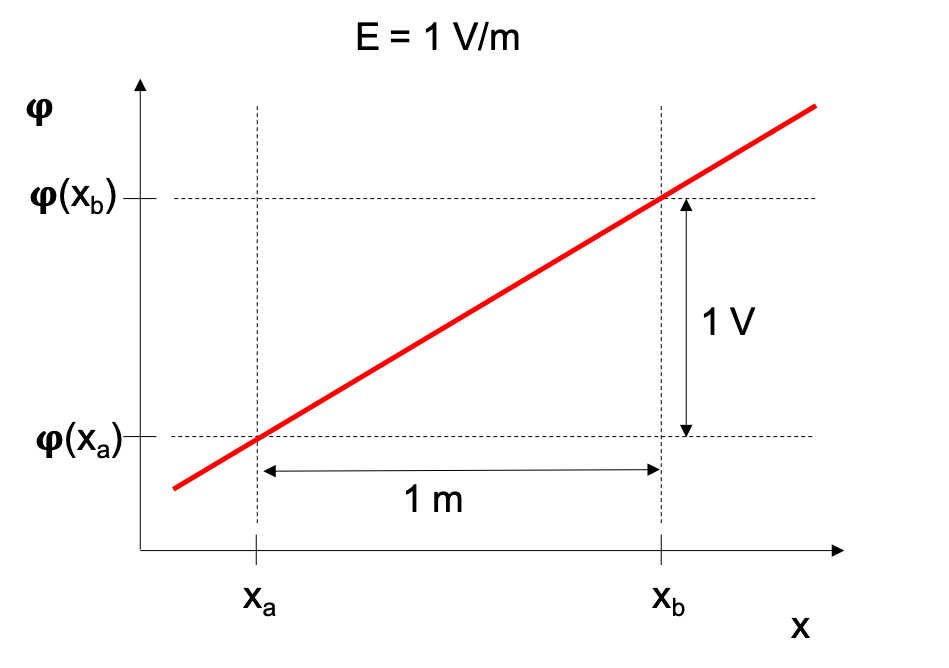
\includegraphics[width=0.8\textwidth]{Figures/Basics/Ground.png}
\end{center}
\caption{\textbf{Relationship between the electric field and electric potential.} With a constant electric field $E = 1$ V/m, the electric potential $\phi$ increases linearly with distance $x$. With two locations $x_a$ and $x_b$ 1 m apart, we know that $\phi(x_b) = \phi(x_a) + 1$ V. We are free to define an arbitrary reference point (ground) for the $\phi$, and if we take $\phi(x_a) = 0$, it follows that $\phi(x) = (x-x_a) \times E$. In $x_b$, we then get $\phi(x_b)=$(1m)$\times$1V/m$=1$ V. Equivalently, we might define $x_b$ as our reference point, which would mean that $\phi(x_b) = 0$ and $\phi(x_a) = -1$ V. Regardless of where we place our reference point, the physics (i.e., the field, $E$) would be the same.
}
\label{Basics:fig:Ground}
\end{figure}

We may use the example in Fig. \ref{Basics:fig:Ground} to define the important concept of \textit{ground}. The field ${\bf E}$ generally determines the potential only up to a constant. In the example, the field $E = 1$ V/m would be consistent with any pair of potentials $\phi_a$ and $\phi_b$ as long as $\phi_b - \phi_a =  1$ V. Since it is the field, and not the potential, that is the fundamental physical entity, we can therefore not speak of the potential in a certain point as an absolute entity, but only the potential \textit{difference} between two points. When we record potential in a given location, we must always record it relative to some an arbitrary reference point, which we call \textit{ground}, and where we define $\phi = 0$ (cf. example in Fig. \ref{Basics:fig:Ground}). 

When we record extracellular potentials, we can chose to place the reference electrode either outside or inside brain tissue \cite**{Sharott2015}, but we typically want to keep it at some distance from the recording electrode, so that reference electrode is not affected by the processes that we investigate with the recording electrode. 

By definition, the electric potential is the energy needed to move a unit of electric charge $q$ from the reference point (ground) to a specific location in the electric field. The unit (V) of the electric potential is equivalent to energy per charge, or Joule per Coulomb (V = J/C). As such, the concept of an electric potential is closely related to the concept of a potential energy. The potential energy ($U_E$) of a charge $q$ in an electric field is:
\begin{equation}
U_E = q\phi.
\label{Basics:eq:UE}
\end{equation}


%%%%%%%%%%%%%%%%%%%%%%%%%%%%%%%%%%%%%%%%%%%%%%%%%
\section{\orange{GH: Electric currents}}
\label{sec:Basics:Current} \index{Electric current}
As we have emphasized several times, we normally do not want to study a macroscopic system by keeping track of individual charges. We are instead interested in the electric currents, $I$ (units Ampere: A = C/s), which represents the net movement of charge at a coarse-grained (space averaged) scale. There exist various kinds of electric currents, differing in terms of what drive them. Here, we shall briefly introduce three kinds, the conductive current, the capacitive current and the diffusive current.


\subsection{\orange{GH: Conductive currents}}
A conductive material  \index{Conductor} is one which charges can move freely through when exposed to an electric field. The conductive current is then defined as the amount of charge that moves through some reference cross-section area per second. 

When dealing with an electric circuit, currents are essentially one dimensional, running in the directions defined by the electric cables. The reference cross-section area is then typically taken to be that of "a whole cable", so that the current simply represents the total current through the cable. A simple example is shown in Fig. \ref{Basics:fig:Currents}A, where a current passes through a cable with a resistor. The current is then given by Ohm's law:
\begin{equation}
I = - \frac{\Delta \phi}{R}, 
\label{Basics:eq:Ohm_R}
\end{equation}
where $\Delta \phi = \phi_B-\phi_A$ is the voltage difference across the resistor, and $R$ (units Ohm ($\Omega$)) its resistance. The cable itself was assumed to have a zero resistance. That means that the entire resistance in the system, and the entire voltage drop, was that over the resistor. To describe this system, we then only needed to consider the potential at two locations, A and B, representing the two sides of the resistor. 

\begin{figure}[!ht]
\begin{center}
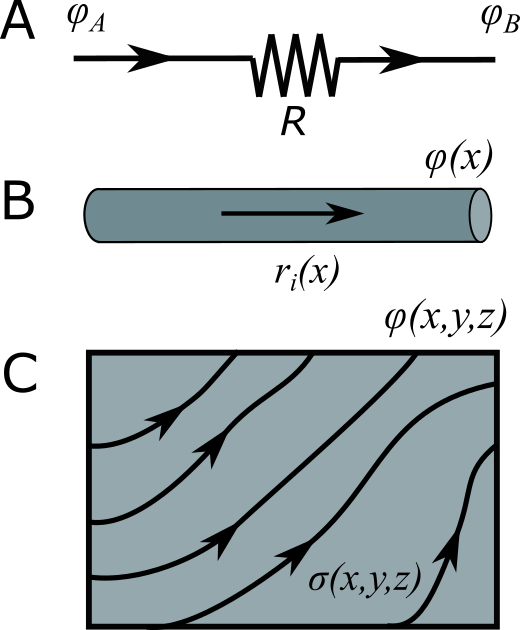
\includegraphics[width=0.6\textwidth]{Figures/Basics/Currents.png}
\end{center}
\caption{{\bf Ohms law for currents and current densities.} {\bf (A)} Current through cable with resistor with resistance $R$ ($\Omega$): $I = (\phi_B-\phi_A)/R$. {\bf (B)} Current in cable with specific axial resistance per unit length $r_a$ ($\Omega$/m).  $I=- (1/r_a) d\phi/dx$. {\bf (C)} Current density (units A/m$^2$) in a volume conductor with conductivity $\sigma$ (Sm): ${\bf i} = \sigma {\bf E} = - \sigma \nabla \phi$.}
\label{Basics:fig:Currents}
\end{figure}

In reality, the resistance of the cable is not strictly zero, although for most electrical circuits this is an excellent approximation. However, in some applications, for example for very long and thin cables, or for cables of less conducting materials, it may be necessary to treat cables as continuous resistors. If we define the specific axial resistance per unit length $r_{a}$ ($\Omega$/m), Ohm's law becomes: 
\begin{equation}
I = - \frac{1}{r_a}\frac{d\phi}{dx}, 
\label{Basics:eq:Ohm_r}
\end{equation}
where $r_a=r_a(x)$ may in principle vary along the cable (Fig. \ref{Basics:fig:Currents}B). With eq. \ref{Basics:eq:Ohm_r}, the potential $\phi(x)$ will vary gradually along the cable. If $r_a$ is constant along the cable, and the cable has length $L$, it is related to the resistance of the total cable through $r_a=R/L$. Conductive currents running axially through neural dendrites and axons are typically modeled in this manner. 

Both examples above were one-dimensional in the sense that the current was restricted to run exclusively in the direction defined by the cable. In a three dimensional volume, such as for example brain tissue, currents may run in all spatial directions (Fig. \ref{Basics:fig:Currents}C). It is then convenient to describe them in terms of a current density, ${\bf i}$,  a vector which defines the current per unit cross section area (units A/(m$^2$) and its spatial direction. The current density can be defined in all points in 3D space, and is not dependent on any particular and predefined cross-section area. The conductive properties of a material can be specified either through its resistivity $r$ ($\Omega$ m), or its inverse, the conductivity $\sigma$ (S/m), both being material properties. We shall here use the latter convention, and with that, Ohms law can be written as:
\begin{equation}
{\bf i} = - \sigma \nabla \phi
\label{Basics:eq:Ohm_3D_phi}
\end{equation}

On a more general form, Ohms law states that:
\begin{equation}
{\bf i} = \sigma {\bf E}, 
\label{Basics:eq:Ohm_general}
\end{equation}
while eqns. \label{Basics:eq:Ohm_R}-\ref{Basics:eq:Ohm_3D_phi} hold only in the case where the electric field ${\bf E}$ is conservative (cf. eq. \ref{Basics:eq:EV}), which we shall assume throughout this book, and which we discuss further in Section \ref{sec:VC:quasistatic}. We note however, that Ohms law applies specifically to \textit{conductive} currents, and that there exist other forms of electric currents not described by it.


\subsection{\orange{GH: Capacitive currents}}
In the theory of electric circuits, a common circuit element is the capacitor. Capacitors are devices that can store electrical energy in terms of an electric field. The simplest form of a capacitor consists of two electrical metallic plates or surfaces separated by an insulating (dielectric) medium \index{Dielectricum}.  By definition, a dielectric medium is one where charges are bound to stay in confined regions of space. An electric field only will slightly shift their average equilibrium positions, causing a polarization of the material.

An illustration of a capacitor is given in Fig. \ref{Basics:fig_Capacitor}. When an electric current $I_{left}$ enters the capacitor from the left, it leads to an accumulation of charge $+q$ on the metal plate on the left hand side of the capacitor. This, in turn, evokes an electric field $\bf E$ across the dielectric material that separates the plates, which drives positive charges away from the rightmost metal plate, leaving it negatively charged $-q$. 

\begin{figure}[!ht]
\begin{center}
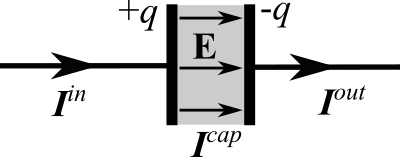
\includegraphics[width=0.6\textwidth]{Figures/Basics/Capacitor.png}
\end{center}
\caption{{\bf Capacitor}.  
}
\label{Basics:fig:Capacitor}
\end{figure}

Whereas the conductive currents $I_{left}$ and $I_{right}$ are mediated by charges moving freely through the cable, no charges actually move across the capacitor itself. However, temporal rate of change of the electric field amounts to a so-called capacitive current  ($I_{cap}$), which is so that current continuity is preserved, i.e., so that $I_{left} = I_{cap} = I_{right}$. The capacitive current is given by: 

\begin{equation}
I_{cap} = C\frac{d\phi}{dt}, 
\label{Basics:eq:Icap}
\end{equation}
where $C$ (units Farad (F=C/V)) is the capacitance. Although $I_{cap}$ differs from conductive currents in the sense that it does not involve free transfer of charge through a medium, it has the same units (A). 

The capacitive current was introduced here because neural membranes have capacitive properties, which causes the neural membrane potential to changes when currents go in or out through the membrane. It custom to express the capacitive membrane current in terms of a current density: 

\begin{equation}
i_{cap} = c_m\frac{d\phi_m}{dt}, 
\label{Basics:eq:Icap_mem}
\end{equation}
where $c_m$ (F/m$^2$) is the capacitance per unit membrane area. In this case, the current density is one-dimensional and in the direction normal to the membrane.


\subsection{\orange{GH: Diffusive currents}}
\index{Diffusion} \index{Electrodiffusion}
The charge carriers in the brain are ions floating around in the salt water solutions that fill up the intra- and extracellular spaces. Ions in salt water will, like electrons in a metal conductor, be accelerated by the presence of an electric field, and will thus carry conductive currents. However, unlike electrons in the metal conductor, ions in water may also move due to diffusion. 

The electrodiffusive nature of ionic motion is described by the Nernst-Planck equation:
\begin{equation}
{\bf j_k} = - D_k {\bf \nabla} c_{k} - \frac{D_k z_k c_k}{\psi} {\bf \nabla} \phi,
\label{Basics:eq:JNP}
\end{equation}
for the flux density, ${\bf j_k}$ (units $mol/\mathrm{m^2s}$), of an ion species $k$. 

The first term on the right hand side of eq. \ref{Basics:eq:JNP} is Fick's law for diffusion. It states that the diffusive flux of ion species $k$ is proportional to the diffusion constant ${D}_k$ (units $\mathrm{m^2/s}$) times the concentration gradient ${\bf \nabla} c_{k}$. ${D}_k$ is generally a property of the medium that the ion diffuses through, and determines how "easy" it is for the ion $k$ to move through the medium. The second term on the right hand side of eq. \ref{Basics:eq:JNP} accounts for ionic drift due to the electric field. The factor $D_k/\psi$ is the electrical mobility of the ions, which is linearly related to their diffusion constant. This linear relationship is called the Einstein relation\index{Einstein relation}. It does not apply generally, but is valid for dilute solutions such as the saline solutions in the brain \cite**{Grodzinsky2011}. $z_{k}$ is the valency, i.e., the number of unit charges associated with of ion species $k$. The factor $\psi=RT/F$ (units V) is defined by the gas constant ($R$), Faraday's constant ($F$) and the temperature ($T$). 

Faraday's constant, $F$, has units C/mol, and is defined as the charge per mol of unit charges. A flux density ${\bf j_k}$ can thus be converted to a current density by multiplying it with $Fz_k$. A salt water solution is composed of several ions, and to obtain the net electric current, we must sum over the contributions from all of them to obtain the total current density: 
\begin{equation}
{\bf i} = \sum_k z_k F {\bf j_k} = -\sum_k{F z_k \tilde{D_k}{\bf \nabla} c_{k}} - F\sum_{k} \frac{\tilde{D_k} z_{k}^2}{\psi}c_{k} {\bf \nabla}{\phi}.
\label{Basics:eq:iNP}
\end{equation}

The last term on the right hand side is the drift current density, 
\begin{equation}
{\bf i}^{drift} = - F\sum_{k} \frac{\tilde{D_k} z_{k}^2}{\psi}c_{k} {\bf \nabla}{\phi} = - \sigma {\bf \nabla}{\phi}.
\label{Basics:eq:idrift}
\end{equation}
As we indicated with the last equality, the drift current density is the same as the Ohmic current that we defined in eq. \ref{Basics:eq:Ohm_3D_phi}, which means that we can identify the conductivity $\sigma$ of a salt water solution as \cite**{Koch1999}:
\begin{equation}
\sigma = \frac{F}{\psi}\sum_{k} \tilde{D}_k z_{k}^2 c_{k},
\label{Basics:eq:sigma_conc}
\end{equation}

The first term on the right hand side of eq. \ref{Basics:eq:iNP} is the diffusive current density, 
\begin{equation}
{\bf i}^{diff}  = -\sum_k{F z_k \tilde{D_k}{\bf \nabla} c_{k}}.
\label{Basics:eq:idiff}
\end{equation}
Hence, in a conductive medium that contains concentration gradients, the total current is not purely Ohmic, but can contain an additional contribution from ionic diffusion. In many cases, the total current will be dominated by the drift component, and it is common to assume that the diffusive component is negligible. 

\subsection{\orange{GH: A note on Ohms law}}
It is important to remember that the current given by eq. \ref{Basics:eq:Ohm_3D_phi} represents the average movement of charge on a coarse-grained level, and does not apply on a microscopic scale. If we compare it with the microscopic fundament for this movement, it is easy to get confused, so let us dive into that confusion and try to clear it up. According to eq. \ref{Basics:eq:E}, an electric field will act on a reference charge $q$ by a constant force, which according to Newton's law (${\bf F} = m{\bf a}$) should give it a constant acceleration in the field-direction. Conversely, eq. \ref{Basics:eq:i} states that ${\bf E}$ gives rise not to a constant acceleration of charges, but rather a constant current, i.e., a constant average \textit{velocity} of charges. 

The reason for the discrepancy between the microscopic (constant acceleration) and macroscopic (constant velocity) level is that the constant acceleration (eq. \ref{Basics:eq:E}) at the microscopic level will go on for only a tiny time period (called the charge relaxation-time) \index{Charge-relaxation} before our protagonist charge $q$ will bump into some other particle and be scattered out in some random direction. After the scattering event, the acceleration will start "from scratch", and go on until the next collision takes place, and so forth. Whereas the scattering events will tend to make the motion of $q$ a random walk (which should give it a zero average velocity in any preferred direction), the small periods of acceleration between collisions will at average give $q$ a net drift velocity in the field direction. As the same will happen for all other charges present, there will be a net drift of charge in the field direction. The current density given by Eq. \ref{Basics:eq:Ohm_3D_phi} is therefore often referred to as the drift current density. Admittedly, the explanation that we proposed here was somewhat hand-waving, and the fact that we get the linear (constant velocity) relationship in eq.\ref{Basics:eq:Ohm_3D_phi} is constitutive, meaning that it is observed experimentally rather than derived from first physical principles, and is found to be a good approximation for many mediums, brain tissue included, under many conditions \cite**{Nunez2006,Pettersen2012}. 


\section{\orange{GH: Electric currents in the brain}}
\label{Basics:braincurrents}
Having introduced three different kinds of currents above, we are now ready to summarize the role that they play within a brain-specific context. It is useful to make a distinction between currents existing in one of three different mediums, running through either: 
\begin{itemize}
\item the intracellular saline solution (cytosol)
\item the extracellular saline solution
\item the cellular (neuronal or glial) membrane
\end{itemize}

Among these three, the membrane currents are the odd ones out. A bit cartoonishly, we may think of the cellular membrane as an insulator (dielectric medium) with small holes \index{Dielectricum}. Due to its dielectric properties, the membrane can store charges in so-called Debye-layers on its the in- and outside in a way equivalent to how charges are stored on the metal plates in a capacitor (cf. Fig.\ref{Basics:fig:Capacitor}). This charge-storage process can be described in terms of a capacitive current like that defined in eq. \ref{Basics:eq:Icap_mem}, which causes the membrane potential to vary. The holes represent various kinds of ion channels, which are conductive pores in the membrane that allow ions to pass through them. Ionic currents through the ion channels come in addition to the capacitive current. Both are essentially one-dimensional, i.e., in the direction perpendicular to the membrane. The ionic currents generally depend both voltage- and ion concentration differences between the inside and outside of the membrane, and are thus electrodiffusive in their nature (cf. eq. \ref{Basics:eq:iNP}, but in one dimension, i.e., $\nabla /rightarrow d/dz$.) 

The intra- and extracellular currents are generally three dimensional electrodiffusive volume currents (cf. eq. \ref{Basics:eq:iNP}) through the conductive saline solutions that fill up the intra- and extracellular spaces. However, as concentration gradients within the intracellular and extracellular spaces typically are much smaller than those across membranes, it is common to neglect the diffusive component, and approximate that intra- and extracellular currents as being purely Ohmic (cf. eq. \ref{Basics:eq:Ohm_3D_phi}). For the intracellular current it is common to make the further simplification that it is well approximated as one-dimensional (cf. eq. \ref{Basics:eq:Ohm_r}). This is motivated by the morphological structure of neurons, which to a fair degree of accuracy can be represented as one-dimensional branching cables of varying diameter.

An illustration of the involved currents in a small piece of tissue is given in Fig. \ref{Basics:fig:Twostep}A. As indicated there, currents travel in loops, so that the intracellular and extracellular currents are coupled through the transmembrane currents at the boundary. Of course, there are infinitely many such loops in the system, and only a few were included in the illustration. 

\begin{figure}[!ht]
\begin{center}
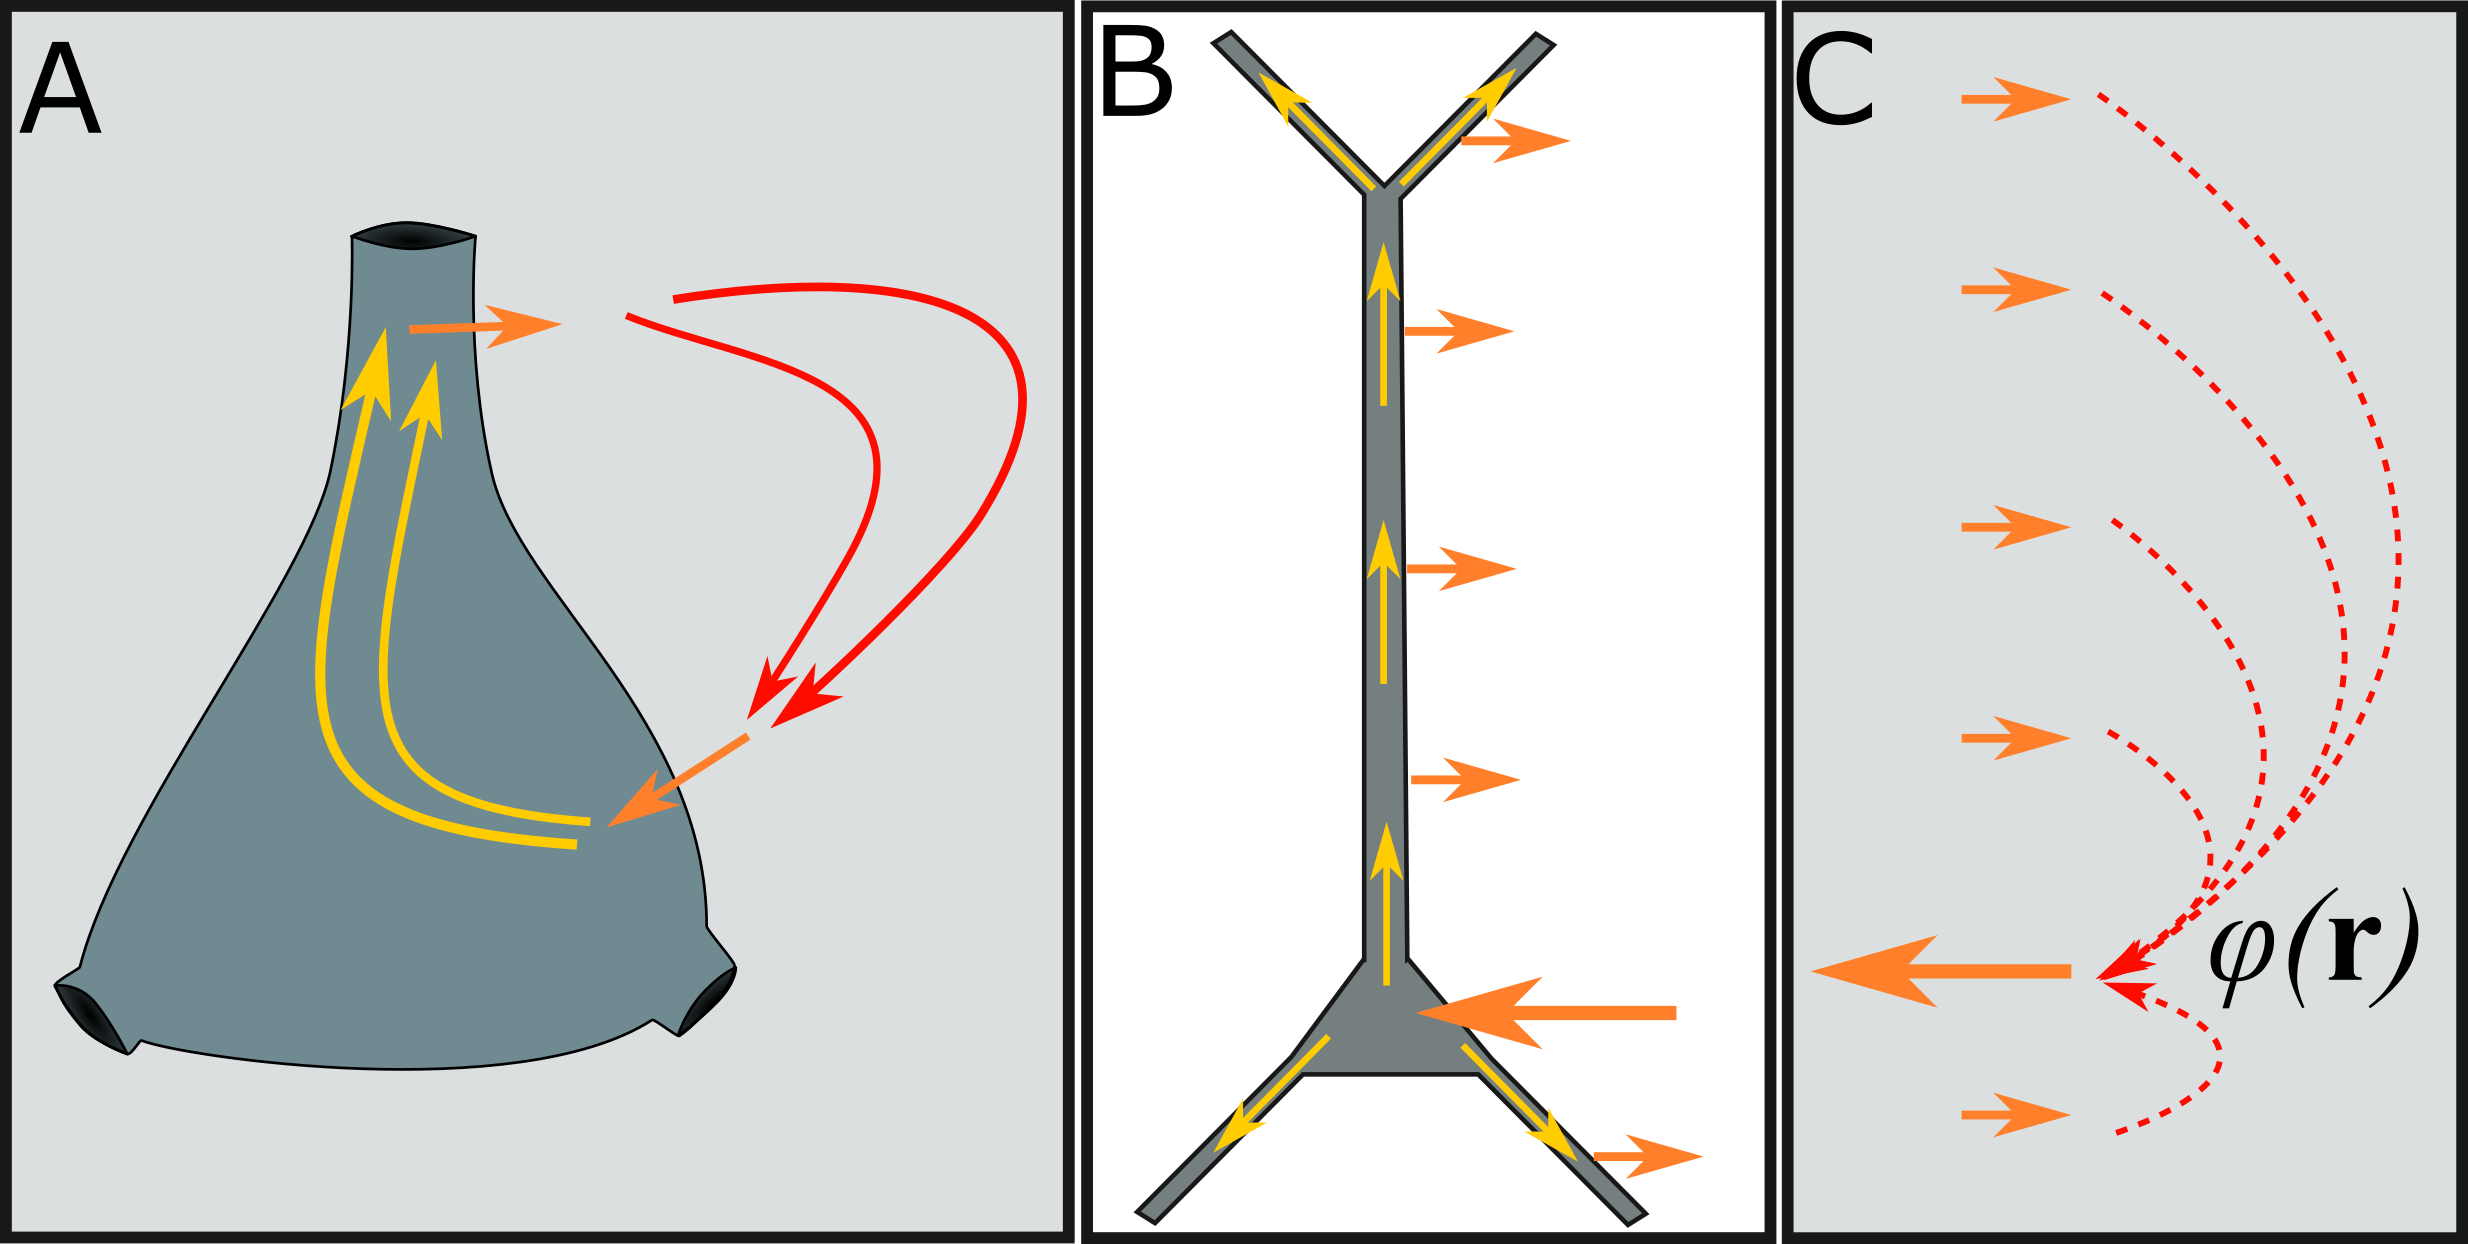
\includegraphics[width=1.0\textwidth]{Figures/Basics/Twostep.png}
\end{center}
\caption{{\bf Currents in brain tissue}. {\bf(A)} Illustration of currents involved in the brain, with intracellular volume currents (yellow), extracellular volume currents (red), and transmembrane currents (orange). Currents travel in closed loops. The entire space will be filled with currents, and only a paths was included in the illustration. {\bf(B)} A standard modeling strategy is to compute the intracellular and transmembrane currents on a framework independent of the extracellular dynamics. The neuron is approximated as a branching cable, and intracellular currents are one-dimensional along the cable, whereas transmembrane currents are perpendicular to the cable and distributed over the cable. {\bf(C)} The transmembrane currents computed in the framework {\bf(B)} can be used as output sources and sinks to the extracellular space, and can be used to compute the extracellular potential $\phi({\bf r})$. This will be the potential that is "needed" to complete all current loops. A few of which are illustrated with red, dashed arrows. 
}
\label{Basics:fig:Twostep}
\end{figure}


\subsection{\orange{GH: Extracellular potentials}}
\label{sec:Basics:ECSpot}
The main focus in this book will be on the modeling and interpretation of extracellular potentials in the brain. In Section \ref{sec:Basics:Fields} we explained that electric fields, and thus electric potentials, ultimately are due to a distribution of charges. However, in neuroscience we rather see extracellular potentials as reflecting transmembrane currents from neurons (and glial cells). The following subchapters will provide some clarity as to why this is the case. 


\subsection{\orange{GH: Electroneutrality of brain tissue}}
\label{sec:Basics:Electroneutrality}
Due to the Coulomb force (eq. \ref{Basics:eq:CoulombF}), positive charges will repel other positive charges, and attract negative charges. An effect of this is that positive charges in a conductive medium will tend to surround themselves with negative charges, and vice versa. Consequently, the numbers of positive and negative charges in a finite volume of space tends to be in balance, and any finite reference volume of brain tissue will, on the coarse-grained scale, be practically electroneutral \cite**{Nunez2006,Grodzinsky2011}. If this were not the case, and a volume did contain a net charge density $\rho$, the very strong Coulomb-forces associated with it would cause $\rho$ to decay to zero at a rate proportional to the so-called \textit{charge-relaxation time}, which in brain tissue is in the order of a nanosecond \cite**{Grodzinsky2011}. 

The Coulomb force also gives rise to a phenomenon called Debye shielding \cite**{Nunez2006}. As positive charges will tend to surround themselves with negative charges, and vice versa, they will tend to shield (cancel out) the electric fields from one another, so that neither of them give any contribution to the field measured at some distance away from the charges.

Of course, a non-zero electric field or potential does require some charge separation somewhere. In the brain, this predominantly happens at the capacitive neuronal membranes, and then on a very small spatial scale. As we described earlier, a patch of membrane has the capacity to separate a charge $q$ on the interior side from a charge $-q$ on the exterior side. However, since the membrane is just some nanometers thick, the two charges $-q$ and $q$ are very close in space, and will shield each others' contributions to extracellular fields measured at some distance from the membrane. 

The practical implication of electroneutrality and shielding effects is that, when we study extracellular potentials (or fields), we can neglect contributions from any particular distribution of charges, and instead compute extracellular potentials from the constraint that there should be no charge accumulation anywhere in the extracellular space. 


\subsection{\orange{GH: Neurons as current sources}}
\label{sec:Basics:C} 
\index{Current source density}
Due to the shielding effects explained above, the sources for the extracellular potential (of field) will exclusively be the electric \textit{currents} entering or leaving the extracellular space through neural membranes. Mathematically, we can express this through the continuity equation:
\begin{equation}
\nabla \cdot {\bf i_t} = -C.
\label{Basics:eq:continuity1}
\end{equation}
where the source term, $C$, is called the current source density (units A/m$^3$), and represents  the transmembrane output currents from neurons per tissue volume. Here, we have let ${\bf i_t}$ denote the density of current running extracellularly through brain tissue. It does not include intracellular or transmembrane neural currents. 

Eq. \ref{Basics:eq:continuity1} tells us that in a volume of space where there is no neuronal membrane ($C = 0$), we have that $\nabla \cdot {\bf i_t} = 0$. This means that there will be no net current entering or leaving such a volume. Importantly, this does not mean that the current must be zero. Currents can and will still run \textit{through} the volume, as long as the amount of current entering it and leaving it are in balance. 

In a volume that \textit{does} receive a neuronal output, eq. \ref{Basics:eq:continuity1} tells us that the current outputted from the neuron into that volume ($C$) must be carried away from that volume in terms of an extracellular tissue current. As we shall show in Chapter \ref{sec:VC}, this conservation law shall be the fundament for modeling extracellular potentials surrounding active neurons.

For most parts of this book, we shall approximate brain tissue as a \textit{linear} Ohmic conductor, which means that the tissue current densities are given by eq. \ref{Basics:eq:Ohm_3D_phi}:
\begin{equation}
{\bf i_t} = - \sigma_t \nabla \phi, 
\label{Basics:eq:i}
\end{equation}
where $\sigma_t$ is the tissue conductivity. Eq. \ref{Basics:eq:i} states that the current density will be proportional to the electric field and the conductivity of the medium, $\sigma_t$. The conductivity is a material property, and in brain tissue, it is often assumed to be a constant, at least within a given brain region. 


\subsection{\orange{GH: Two-step approach for modeling extracellular potentials}}
To compute extracellular potentials based on eq. \ref{Basics:eq:continuity1}, we off course need to know the neuronal output $C$. Generally, the transmembrane currents in neurons depend on the membrane potential $\phi_m$, which is defined as the difference between the intracellular ($\phi_i$) and the extracellular $\phi_e$ potentials immediately inside and outside the membrane. To compute intra- and extracellular potentials on a unified and spatially resolved framework is extremely computationally demanding, and unattainable for any large systems. Standard modeling approaches are therefore based on the simplifying assumption that the neurodynamics is independent of whatever goes on in the extracellular space. One may take a two-step approach to model the cellular and extracellular dynamics: 

\begin{itemize}
\item {\bf Step 1:} Compute the cellular dynamics (intracellular currents, membrane currents, and membrane potential) on a separate framework based on the assumption that this is independent on what goes on in the extracellular space (Fig. \ref{Basics:fig:Twostep}B). 

\item {\bf Step 2:} Use the transmembrane currents computed in Step 1 as "external" input to the extracellular space (Fig. \ref{Basics:fig:Twostep}C). Based on current continuity (eq. \ref{Basics:eq:continuity1} with $C$ as boundary conditions obtained in Step 1, an analytical formula can then be derived for how the set of transmembrane currents give rise to an extracellular potential $\phi({\bf r})$. 
\end{itemize}

Throughout this book, we shall use this two-step approach to compute extracellular potentials, although we will briefly introduce the theory behind more advanced, alternative frameworks. The standard framework for completing Step 1 is presented in Chapter \ref{sec:Neuron}, and the standard framework for completing Step 2 is presented in Chapter \ref{sec:VC}. 



\section{\orange{GH: Maxwell's equations}}
\label{sec:Basics:Maxwell} \index{Maxwell's equations}
Most of the physics that we have gone through so far follows from Maxwell's equations, so we will summarize this chapter by going briefly through these. The equations come in two versions, referred to as the microscopic and macroscopic versions. The microscopic version is the most fundamental, but using it requires knowledge of the positions of all individual charges. Since that is unfeasible when any medium at a macroscopic level, we therefore only list up the macroscopic set of equations: 

\begin{eqnarray}
\nabla\cdot {\bf D} & = & \rho. \label{Basics:eq:Max11} \\
\nabla \cdot {\bf B} & = & 0.  \label{Basics:eq:Max22} \\
\nabla \times {\bf E} & = & - \frac{\partial {\bf B}}{\partial t}.  \label{Basics:eq:Max33} \\
\nabla \times {\bf H} & = & \bf{i^{free}} + \frac{\partial {\bf D}}{\partial t}.  \label{Basics:eq:Max44}.
\end{eqnarray}

Here $\rho$ and $\bf{i^{free}}$ are the free (unbound) charge and current densities. For linear mediums , the auxillary fields (${\bf H}$ and ${\bf D}$) can be expressed in terms of the fundamental magnetic (${\bf B}$) and electric (${\bf E}$) fields through the constitutive relations ${\bf B} = \mu{\bf H}$ and ${\bf D} = \epsilon {\bf E}$, where $\mu$ is the magnetic permeability of the medium and $\epsilon$ the electric permittivity of the medium. This is an excellent approximation for brain tissue, so that we may write the Maxwell equations at the form:

\begin{eqnarray}
\nabla\cdot {\bf E} & = & \frac{\rho}{\epsilon}. \label{Basics:eq:Max1} \\
\nabla \cdot {\bf B} & = & 0.  \label{Basics:eq:Max2} \\
\nabla \times {\bf E} & = & - \frac{\partial {\bf B}}{\partial t}.  \label{Basics:eq:Max3} \\
\nabla \times {\bf B} & = & \mu\bf{i^{free}} + \mu\epsilon\frac{\partial {\bf E}}{\partial t}.  \label{Basics:eq:Max4}
\end{eqnarray}

\ehnote{Kanskje du boer ta en ekstra titt paa likning 6 spesielt i Hamalainen '93 igjen?}
\ghnote{Hva mener du? Var det den H-en som var problemet, eller ser du andre problemer?}

Eq. \ref{Basics:eq:Max1} is Gauss's law (for electricity). The free charge density, $\rho$, can generally be non-zero, although we argued earlier that brain tissue for practical purposes can be assumed to be electroneutral at the coarse-grained scale. 

Eq. \ref{Basics:eq:Max2} is Gauss's law for magnetism, and is the magnetic equivalent to eq. \ref{Basics:eq:Max1}. Whereas eq. \ref{Basics:eq:Max1} allows a spatial gradient of the electric field due to a local charge density $\rho$, eq. \ref{Basics:eq:Max1} disallows the corresponding gradient in the magnetic induction field. That is because magnetic monopoles do not exist. 

Eq. \ref{Basics:eq:Max3} is the Maxwell-Faraday equation for electric induction. The cross product $\nabla \times {\bf E}$ represents a certain kind of change in the electric field called the \textit{curl}. The equation tells us that such a change will be induced if there is a temporal variation in the magnetic field. 

Eq.  \ref{Basics:eq:Max4} is Ampere's circuital law, and is the magnetic equivalent to eq. \ref{Basics:eq:Max3}. According to eq. \ref{Basics:eq:Max4}, a magnetic field will be induced either by an electric current of free charges going through the medium (first term on the right), or by a temporal change in the displacement field (second term on the right). 

Together, Maxwell's equations give a unified theory for electricity and magnetism, and laid the theoretical fundament for understanding electromagnetic radiation such as light. We can "see the light" by looking at eqns. \ref{Basics:eq:Max3} and \ref{Basics:eq:Max4}. Eq. \ref{Basics:eq:Max3} shows that a temporal change the magnetic field induces an electric field perpendicular to the change (perpendicular, because that is what the operation $\nabla \times$ does). while eq. \ref{Basics:eq:Max4} (last term) shows that a temporal change in the electric field induces magnetic field perpendicular to the change. Electromagnetic radiation is due to such an interplay where electric and magnetic fields act on each-others through a periodic series of inductions and cancellations that propagate as a wave through a medium. 

\subsection{\orange{GH: Quasi-electrostatic approximation}}
For our studies of brain dynamics, electromagnetic radiation does not play an important role. Electric fields do not depend exclusively on magnetic induction, but can according to eq. \ref{Basics:eq:Max1} also be evoked also by the presence of electric charges. In the brain, this latter contribution is much larger than the contribution from magnetic field variations. When studying brain processes, we can therefore apply the so-called electro-quasi-static approximation of Maxwell's equations, which means that the temporal derivative of the magnetic field is assumed to be so small that it as a negligible impact on ${\bf E}$. This means that eq. \ref{Basics:eq:Max3} simplifies to $\nabla \times {\bf E} = 0$, which is a prerequisite for expressing ${\bf E}$ as a gradient of a potential (cf. eq. \ref{Basics:eq:EV}). This assumption was also implicit when we expressed {\bf E} as a function of charges in eq. \ref{Basics:eq:CoulombEN}. 

\subsection{\orange{GH: Quasi-magnetostatic approximation}}
The right hand side of eq. \ref{Basics:eq:Max4} is composed of a current of free charges (first term) plus a so-called displacement current (last term). The capacitive current that we introduced earlier (eq. \ref{Basics:eq:Icap_mem}) is an example of a displacement current, and the capacitance a function of $\epsilon$. The Ohmic current that we introduced earlier (cf. eq. \ref{Basics:eq:Ohm_general}) is an example of a current of free charges. For an idealized conductor, the displacement current is zero, while for an idealized capacitor, the current of free charges is zero. 

Making the quasi-magnetostatic approximation means setting the last term in eq. \ref{Basics:eq:quasimag} to zero. If we assume that the first term is purely Ohmic (cf. eq. \ref{Basics:eq:Ohm_general}), we may write eq. \ref{Basics:eq:Max4}:

\begin{equation}
\nabla \times {\bf B}  =  \mu \left( \sigma {\bf E} + \epsilon\frac{\partial {\bf E}}{\partial t} \right). 
\label{Basics:eq:quasimag}
\end{equation}
The quasi-magnetostatic approximation thus holds if 


so that $\nabla \times {\bf B}  =  \mu\bf{i^{free}}$. This is a good approximation for the extracellular and intracellular currents, but not for the membrane currents, where the last, displacemen term


In a perfect conductor, the last term is zero. 



 while the 
For a perfect conductor, the displacement current is zero, while for a perfect capacitor, the current of free charges is zero. 

The displacement current is directly related to the capacitive cur





From eqns. \ref{Basics:eq:Max1} and  \ref{Basics:eq:Max4} we can derive the concept of charge conservation. If compute the divergence (take $\nabla \cdot$) of both sides of \ref{Basics:eq:Max4}:
\begin{equation}
- \nabla \cdot {\bf i^{free}} =  \epsilon \frac{\partial (\nabla \cdot {\bf E})}{\partial t}, 
\label{Basics:eq:Max4dot}
\end{equation}
and insert eq. \ref{Basics:eq:Max1} on the right hand side, we get:
\begin{equation}
- \nabla \cdot {\bf i^{free}} =  \frac{\partial \rho}{\partial t},
\label{Basics:eq:Max4dot1}
\end{equation}
If the left hand side in nonzero, it means that there will be a net influx of current into a volume, and if that is the case, we must have an accumulation of charge there, as described by the right hand side of the equation. 




The link between eq. \ref{Basics:eq:Max4dot} and the fundamental equation for modeling extracellular potentials (eq. \ref{Basics:eq:continuity1}) is easier to recognize if we define a total current density ${\bf i} = \bf{i^{free}} +\epsilon\partial{\bf E}/\partial{t}$. 

With the displacement current "baked into" a total current in this way, charge conservation implies current continuity:

\begin{equation}
\nabla \cdot {\bf i} =  0,
\label{Basics:eq:Max4dot1}
\end{equation}
Further, we may make a decomposition of ${\bf i} = {\bf i_t} + {\bf i_p}$ into an extracellular tissue component and a primary cellular (intra-cellular + membrane) component. 

\begin{equation}
\nabla \cdot {\bf i_t} =  -\nabla \cdot {\bf i_p},
\label{Basics:eq:Max4dot1}
\end{equation}

Since the currents ${\bf i_t}$ and  ${\bf i_p}$ do not exist at the same point in space (except at the membrane boundary), this equation


$- \nabla \cdot \bf{i^{free}} =  \epsilon \frac{\partial {\bf \nabla \cdot E}}{\partial t}, $


In the case of electroneutrality ($\rho = 0$), eq. \ref{Basics:eq:Max4dot1} reduces to:
\begin{equation}
- \nabla \cdot {\bf i} =  0.
\label{Basics:eq:MaxElectroneutral}
\end{equation}


In the previous subsection, we said that eq. \ref{Basics:eq:continuity1} will be our fundamental equation for modeling extracellular potentials. It is therefore important to point out that it is not in disagreement with Maxwell's equations, although eq. \ref{Basics:eq:continuity1} and eq. \ref{Basics:eq:MaxElectroneutral} at a first glimpse may look a bit different. Comparing the two, we we see that in \ref{Basics:eq:continuity1}, ${\bf i}$ has been replaced with ${\bf i_t}$, and a source term $C$ has been added on the right hand side. Essentially, eq. \ref{Basics:eq:continuity1} thus follows from decomposing the total current ${\bf i}$ in eq. \ref{Basics:eq:MaxElectroneutral} into the part of it ($\bf{i_t}$) that runs extracellularly through the tissue and the part of it ($C$) that enters the extracellular space through neural membranes. The reason for making this decomposition is practical. As we shall see in Chapter \ref{sec:VC}, it makes computations easier.





